\documentclass[conference]{IEEEtran}
\IEEEoverridecommandlockouts
% The preceding line is only needed to identify funding in the first footnote. If that is unneeded, please comment it out.
\usepackage{cite}
\usepackage{amsmath,amssymb,amsfonts}
\usepackage{algorithmic}
\usepackage{graphicx}
\usepackage{textcomp}
\def\BibTeX{{\rm B\kern-.05em{\sc i\kern-.025em b}\kern-.08em
    T\kern-.1667em\lower.7ex\hbox{E}\kern-.125emX}}
\begin{document}

\title{A Research on Semantic Middleware\\

}

\author{\IEEEauthorblockN{Shanliang Yao}
\IEEEauthorblockA{\textit{Department of Computer Science and Software Engineering} \\
\textit{Xi’an Jiaotong-Liverpool University}\\
Suzhou, China \\
Shanliang.Yao19@student.xjtlu.edu.cn}
}

\maketitle

\begin{abstract}
Semantic middleware helps computers better understand the content of the network and greatly promotes the development of the semantic web. This research deeply analyzes the origin and development of semantic web, linked data, and semantic middleware.  It studies the strengths and limitations of the three semantic middlewares of Dubbo, RFID, and Seata, and their applications in the real-world industry. Benefits of these semantic middleware are also discussed in this study which can help practitioners choose the appropriate middleware for their applications.

\end{abstract}

\begin{IEEEkeywords}
semantic middleware, semantic web, linked data, Dubbo, RFID, Seata
\end{IEEEkeywords}

\section{Introduction}
\subsection{Background}

At the beginning of the World Wide Web (WWW), the content on the network was only human-readable, but the computer could not understand and process it. There are pictures and links on the webpage, but the computer does not know what the pictures are about, and it is unclear how the link points to the current page. The Semantic Web is a general framework proposed to make data on the network machine-readable \cite{b1}. Semantic is to express the meaning behind the data in a richer way, so that the machine can understand the data. Web hopes that these data link with each other to form a huge information network, just like the interconnected web pages on the Internet, but the basic unit becomes smaller data.

Linked data was originally used to define how to use Semantic Web technology to publish data on the Internet, which emphasizes the creation of links between different data sets. Linked data uses the Resource Description Framework (RDF) as the data model \cite{b2}. It is a set of technical specifications of markup languages proposed by the World Wide Web Consortium (W3C). It is based on the XML grammar and XML Schema data types in order to describe and express the content and structure of network resources more abundantly. The powerful distributed open graphical data model of Linked Data makes it ideal for integrating data stored in various databases and file systems, as well as integrating applications related to such data.

Middleware is a collection of common parts in the integration process for information system interaction. It shields complex and general functions such as communication, interaction, and connection at the bottom, and is provided in the form of products \cite{b3}. When the system is interacting, middleware is used to connect and interact directly, avoiding a lot of code development and labor costs. Through the middleware, each business system can be separated and bear the pressure alone. Such an architecture ensures the high availability of the project. The emergence of semantic middleware has helped computers better understand the content of the network and greatly promoted the development of the semantic web.

\subsection{Research Question}
The development of semantic middleware is getting faster in the technical field. The use of semantic middleware in practical projects is also of great significance. To gain a deeper understanding of semantic middleware and its function, my research questions are described as follows: 
How to apply semantic middleware to real-world applications and what benefits it can bring to this area.

\section{Literature Review}

There are many types of semantic middleware that can be used to solve various problems for either enterprise or platform purposes. In this research, I mainly review three kinds of middleware, namely Dubbo, RFID and Seata, and explain their strengths and limitations with some technical details.

\subsection{Dubbo}

Dubbo is a high-performance, lightweight service middleware created by Alibaba and can be seamlessly integrated with the Spring framework \cite{b6}. It provides three core capabilities: interface-oriented remote method invocation, intelligent fault tolerance and load balancing, and automatic service registration and discovery.

\subsubsection{Categorization}
\
\newline
\indent
Dubbo is a type of Remote Procedure Call (RPC) middleware which is a process where a client application calls a remote server. Its basic idea is to keep the syntax of the client and server programs the same, as if they were on the same machine. The application calls the remote procedure just like the local procedure, starts the operation of the remote procedure, and then returns the result of the operation to the local procedure \cite{b7}.

\subsubsection{Strengths}

\paragraph{High-performance RPC call for interface proxy}
Dubbo provides high-performance agent-based remote calling capabilities, services with an interface as the granularity, shielding developers from the underlying details of remote calls.

\paragraph{Intelligent load balancing}
It has built-in multiple load balancing strategies to intelligently sense the health status of downstream nodes, significantly reduce call delays, and improve system throughput.

\paragraph{Service automatic registration and discovery}
This middleware supports multiple registration center services, and real-time service instance online and offline perception.

\paragraph{Highly scalable}
Dubbo follows the design principles of microkernels and plug-ins. All core capabilities such as Protocol, Transport, and Serialization are designed as extension points, treating built-in implementations and third-party implementations equally.

\paragraph{Traffic scheduling during operation}
It has built-in routing policies such as conditions and scripts. By configuring different routing rules, it is easy to implement gray-scale publishing and priority in the same computer room.


\subsubsection{Limitations}
\
\newline
\indent
Although Dubbo has many strengths and can handle many problems in different scenarios, it still has some disadvantages.

\begin{itemize}
\item Dubbo has insufficient support for languages, and currently only supports JAVA.

\item The coding development of Dubbo is difficult, because the dependency of Dubbo's jar package can not be solved by many large projects.
\end{itemize}


\subsection{RFID}

The RFID middleware is located between the RFID system and the application system, and is responsible for data transmission between the RFID system and the application system.
It is responsible for solving the problems of reliability, security and data format conversion of RFID data.

The connection between the RFID middleware and the RFID system is implemented using the application program interface (API) provided by the RFID system \cite{b8}. After the data in the RFID card is read by the reader, it is transmitted to the RFID middleware through the API program. After the RFID middleware processes the data, it publishes the data externally through standard interfaces and services.

\subsubsection{Categorization}
\
\newline
\indent
RFID middleware is a kind of Message-Oriented Middleware (MOM). Information is transmitted in the form of a message from one program to another program or multiple programs \cite{b9}. MOM contains functions not only for passing information, but also for interpreting data, security, data broadcasting, error recovery, locating network resources, finding paths that meet costs, prioritizing messages and requirements, and other services.

\subsubsection{Strengths}

\paragraph{Insulation Infrastructure}
RFID middleware is independent and interposed between RFID readers and back-end applications, and can be connected to multiple RFID readers and multiple back-end applications to reduce the complexity of architecture and maintenance \cite{b10}.

\paragraph{Data Flow}
The main purpose of RFID is to convert physical objects into virtual objects in the information environment, so data processing is the most important function of RFID. RFID middleware has the characteristics of data collection, filtering, integration and transmission, to pass the correct object information to the enterprise's back-end application system.

\paragraph{Process Flow}
RFID middleware uses program logic and store-and-forward functions to provide sequential message flows, and has the ability to design and manage data flows.

\paragraph{Standard}
RFID is an application of automatic data sampling technology and the identification of physical objects. The Electronic Product Code (EPC) is stored in the RFID, and after being read by the RFID reader, it can provide the tracking of the item name and related information represented by the EPC, and immediately identify and share the item data in the supply chain, effectively providing information transparency.

\subsubsection{Limitations}
\
\newline
\indent
 At present, the main suppliers of RFID middleware platforms are IBM, Oracle, Microsoft, SAP, and Sun. For these manufacturers, RFID middleware is just an extension of their existing software, and their RFID products can be quickly and easily integrated with their respective existing software product lines. But it also has some limitations, such as that its products depend on other vendors' software products. Besides, the cost of RFID is too high, coupled with the high cost of RFID transmitters, readers, encoders and antennas.
 
 
 \subsection{Seata}

Seata is an Alibaba open source distributed Transaction Processing Middleware (TPM), to provide high-performance and easy-to-use distributed transaction services under the microservice architecture.

Seata's design idea is that a distributed transaction can be understood as a global transaction. A branch transaction is a local transaction that satisfies atomicity, consistency, isolation, and durability (ACID) \cite{b11}. Therefore, we can operate distributed transactions just like local transactions.



\begin{figure}[h]
\centering
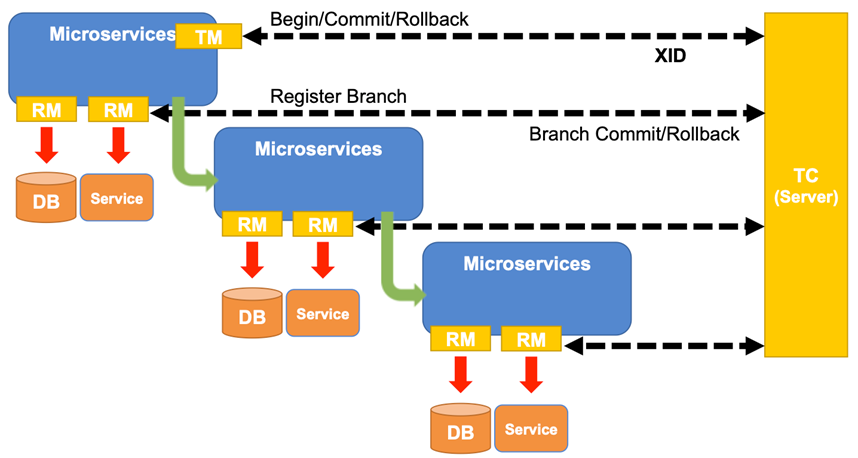
\includegraphics[width=1\columnwidth]{seata}
\caption{Execution process of distributed transactions.}
\label{fig}
\end{figure}

\subsubsection{Technical Detail}
\ 
\newline
\indent 
As shown in Fig. 1, there are three major modules in Seata, namely Transaction Manager (TM), Resource Manager (RM) and Transaction Coordinator(TC). Among them, TM and RM are integrated as Seata's client and business system, and TC is independently deployed as Seata's server.



In Seata, the execution process of distributed transactions \cite{b12}:

\begin{itemize}
\item TM starts distributed transactions (TM registers global transaction records with TC).
\item According to the business scenario, arrange resources such as databases and services (RM reports resource preparation status to TC).
\item TM ends the distributed transaction, and the transaction ends in one phase (TM notifies TC to commit/roll back the distributed transaction).
\item TC summarizes the transaction information and decides whether the distributed transaction is committed or rolled back.
\item TC informs all RMs to commit/roll back resources, the second phase of the transaction ends.
\end{itemize}


\subsubsection{Strengths}
\paragraph{No impact on business}
The impact here refers to the design and transformation of applications at the business level due to the constraints of the technical issue of distributed transactions. This design and modification often bring high research and development and maintenance costs to the application. Solving the distributed transaction problem at the middleware level does not require the application to do extra work at the business level.

\paragraph{High performance}
High performance: Introducing the guarantee of distributed transactions, there will inevitably be additional overhead, causing performance degradation. Reduce the performance loss introduced by distributed transactions to a very low level, so that applications will not be affected by the availability of services due to the introduction of distributed transactions.

\subsubsection{Limitations}
\
\newline
\indent
Seata can only be used in relational databases that support ACID.
The transaction isolation level supports up to the level of read submission, and the analysis of SQL cannot cover all the syntax.

\section{Analysis and Discussion}

I have performed research on the real-world applications and systems in different areas that make use of the semantic middleware. In this chapter, I enumerate three industries in which semantic middleware plays an important role.

\subsection{E-commerce system}

Micro-services are widely used in e-commerce systems. It advocates the division of monolithic applications into a set of several small services. The services coordinate and cooperate with each other to provide users with e-commerce services.

\subsubsection{Use of middleware}
\
\newline
\indent
Dubbo is Alibaba's open source distributed service middleware and is widely used by various Internet companies. The maturity of Dubbo middleware itself and the completeness of documents can basically meet the business needs of various Internet companies. Distributed application scenarios have high concurrency, high scalability and high-performance requirements. It also involves serialization, deserialization, networking, multithreading, and design patterns. Fortunately, the Dubbo framework encapsulates the above knowledge, allowing programmers to focus on the business.

\begin{figure}[h]
\centering
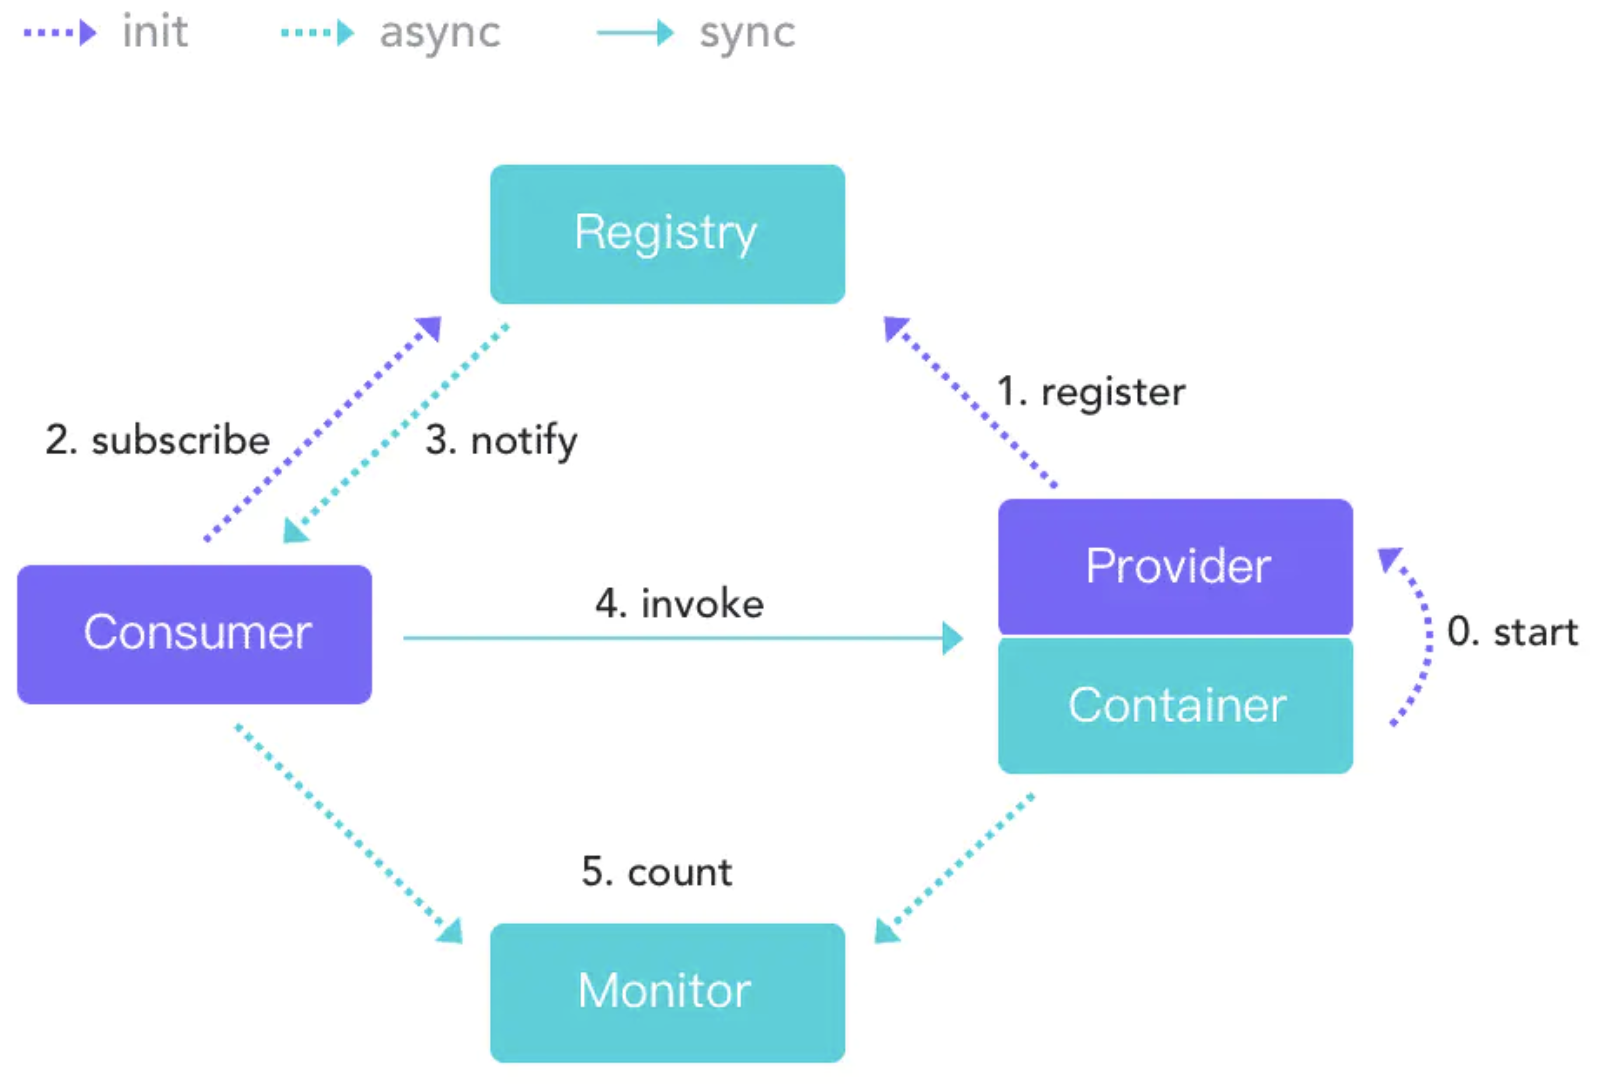
\includegraphics[width=1\columnwidth]{dubbo}
\caption{Dubbo architecture.}
\label{fig}
\end{figure}

Fig. 2 above shows the calling relationship of Dubbo.

\begin{itemize}
\item The service container is responsible for starting, loading, and running the service provider.
\item When the service provider starts, it registers its own service with the registration center.
\item Service consumers subscribe to the services they need from the registration center when they start up.
\item The registration center returns the list of service provider addresses to consumers. If there is a change, the registration center will push the changed data to the consumer based on the long connection.
\item Service consumers, from the provider address list, based on the soft load balancing algorithm, select a provider to call, if the call fails, then select another call.
\item Service consumers and providers accumulate call times and call times in memory, and regularly send statistical data to the monitoring center every minute.
\end{itemize}


\subsubsection{Benefits of middleware}
\
\newline
\indent
Dubbo middleware solves complex business scenarios, rapid business growth, and endless stability issues. Dubbo supports all trading and non-transactional business systems of Alibaba Group (Taobao, Tmall), and safely passed the trading challenge of 11.11 shopping festival.
Many other e-commerce platforms also use Dubbo to help their systems run smoothly and provide users with services.

\subsection{Internet of Things}
The proposition of the semantic concept of the Internet of Things stems from the need to solve the heterogeneous interconnection and platform intelligence formed during the rapid development of the Internet of Things \cite{b4}. The IoT semantics describe resources in a semantic way, which makes the description of resources have good readability and is easy for the machine to understand and process, to realize the functions of semantic operations, semantic query, semantic reasoning and semantic combination \cite{b5}.

\subsubsection{Use of middleware}
\
\newline
\indent
Middleware is located between the underlying RFID hardware equipment (such as radio frequency identification reader) and the back-end database and application software (such as the ERP system) in the RFID application system. It filters, summarizes and calculates the tags-related events and data from the reader, reducing the huge amount of raw data transmitted from the reader to enterprise applications

Relying on the powerful functions of RFID technology in identification, perception, networking, positioning, etc., applying it to the management of the manufacturing process of complex parts can enhance the intelligent image of products and improve the quality and service of product design, production, sales, after-sales, and maintenance. Level, to achieve the full life cycle of the product, and effectively improve its manufacturing efficiency and quality.

\subsubsection{Benefits of middleware}
\
\newline
\indent
For application developers, the important function of RFID middleware lies in the powerful event processing and software management mechanism unique to the product. The event processing engine helps developers easily establish, deploy, and manage an end-to-end logical RFID processing process, which is completely independent of the underlying specific device model and information exchange protocol between devices \cite{b13}. Because the mode of logical devices is used in the event processing engine, the RFID data processing process can be truly separated from the physical topology of the devices that the application deployment phase faces, thus greatly reducing the complexity of the design and not having to care about the supply of these devices Quotient and what communication protocol is used between them.

RFID middleware can also be effectively combined with such as Enterprise Resource Planning (ERP) system, warehouse management system (WMS) and other proprietary business systems for business processing \cite{b14}. This good adaptability makes the RFID application built using this framework only need to make a very small amount of program changes to work seamlessly with the original business system software.

\subsection{Finance}
The data consistency requirements of the financial industry are relatively high. That is to say, if a step fails, then either roll back to the previous service call, or keep retrying to ensure that all steps are successful. The business process under the micro-services architecture in the financial field tends to be more complicated and long. For example, it is normal for an Internet micro-loan business process to adjust more than a dozen services, and the process of exception handling is more complicated.

\subsubsection{Use of middleware}
\
\newline
\indent

\begin{figure}[h]
\centering
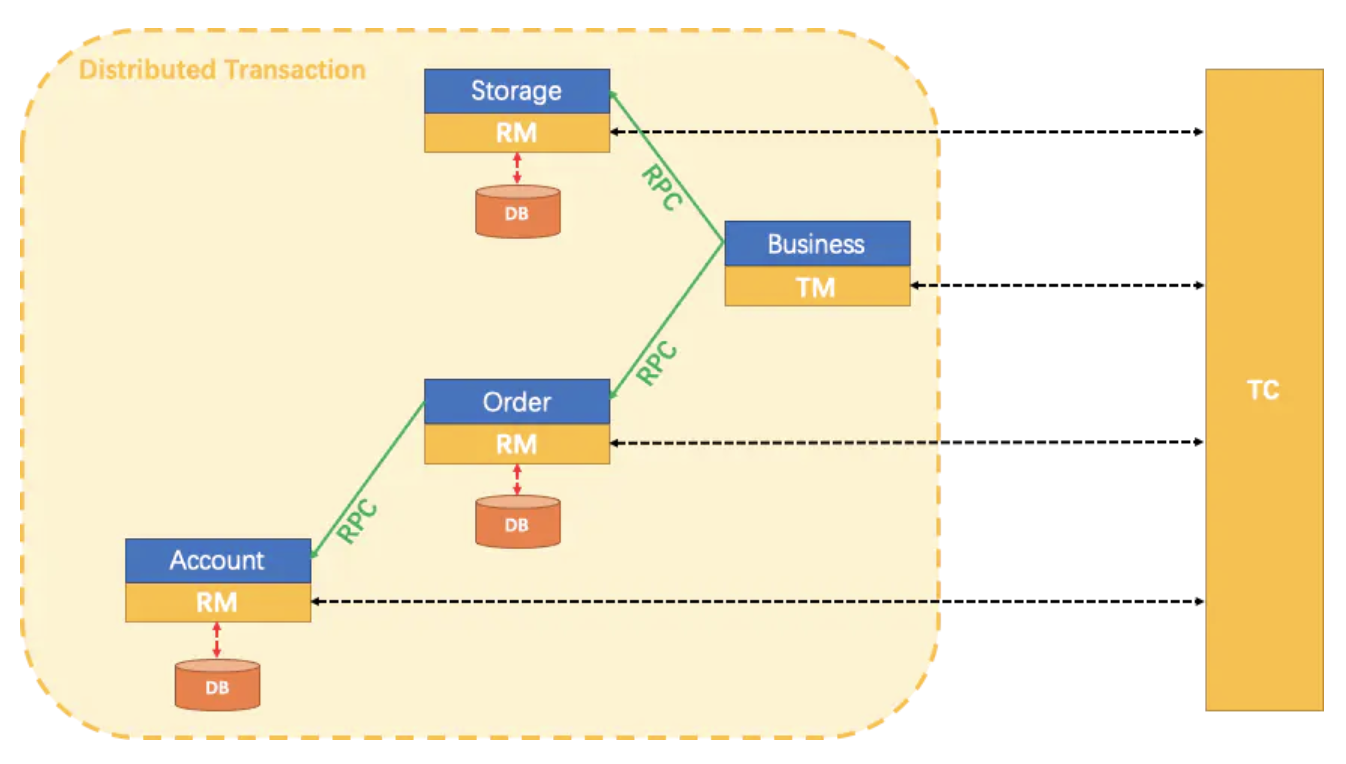
\includegraphics[width=1\columnwidth]{seata2}
\caption{An example of using seata.}
\label{fig}
\end{figure}

Fig. 3 is an example showing a business scenario using Seata. It includes three modules: TM, RM, and TC, and four services: Account, Order, Business, and Storage. The client initiates a business service, and Business calls Storage to lock the inventory and Order to generate an order. Order calls Account to deduct the balance. The roles corresponding to each service are already marked on the icon.


\subsubsection{Benefits of middleware}
\
\newline
\indent
The financial industry must do centralized processing. This is not simply a matter of adding or subtracting amounts. It involves changes in the back-end logical data such as customer accounts, household accounts, and general ledger accounts. All accounting systems must be managed in accordance with the rules. Borrowing and lending must be completed in real time in a logical processing transaction unit and guarantee ACID \cite{b15}.

Seata has been used on Alipay for a long time, and maintains the stable operation of Alipay. When some servers are down, it can still switch to other servers. And when the transaction is abnormal, it still maintains the consistency of the data. It is precise because of Seata's high reliability that its use in the financial field is getting wider and wider.


\section{Conclusion}

\subsection{Summary}
The emergence of semantic middleware has helped computers better understand the content of the network and greatly promoted the development of the semantic web. This research studies the categorization, functions, strengths and limitations of the three semantic middlewares of Dubbo, RFID, and Seata. It analyzes the real-world applications that have used these middleware and the benefits it brings to the industries. This research also provides middleware solutions for similar problems encountered in the industry.


\subsection{Future Work}
After this research, I will continue to study theories and technologies of semantic middleware, and compare the functions and implementation principles of different middleware.

Besides, I will also deeply study its application in the Internet of Things, combine middleware and the Internet of Things, and do some innovative development work to better understand the meaning of middleware in software architecture.




\begin{thebibliography}{00}
\bibitem{b1} Berners-Lee, T., Hendler, J., & Lassila, O. (2001). The semantic web. Scientific american, 284(5), 34-43.
\bibitem{b2} Bizer, C., Heath, T., & Berners-Lee, T. (2011). Linked data: The story so far. In Semantic services, interoperability and web applications: emerging concepts (pp. 205-227). IGI Global.
\bibitem{b4} Katasonov, A., Kaykova, O., Khriyenko, O., Nikitin, S., & Terziyan, V. Y. (2008). Smart Semantic Middleware for the Internet of Things. Icinco-Icso, 8, 169-178.
\bibitem{b3} Lassila, O., & Khushraj, D. (2005, July). Contextualizing applications via semantic middleware. In The Second Annual International Conference on Mobile and Ubiquitous Systems: Networking and Services (pp. 183-189). IEEE.
\bibitem{b5} Terziyan, V., Kaykova, O., & Zhovtobryukh, D. (2010, May). Ubiroad: Semantic middleware for context-aware smart road environments. In 2010 Fifth International Conference on Internet and Web Applications and Services (pp. 295-302). IEEE.
\bibitem{b6} Xiaojun, W., Xu, S., Zhe, H., & Huijuan, L. (2017, May). Research on the Construction of Resource Sharing Platform Based on MicroService. In 2017 International Conference on Smart Grid and Electrical Automation (ICSGEA) (pp. 713-717). IEEE.
\bibitem{b7} Yang, H., Huang, L., Luo, C., & Yu, Q. (2020, April). Research on Intelligent Security Protection of Privacy Data in Government Cyberspace. In 2020 IEEE 5th International Conference on Cloud Computing and Big Data Analytics (ICCCBDA) (pp. 284-288). IEEE.
\bibitem{b8} Minbo, L., & Hua, L. (2011). Research on RFID integration middleware for enterprise information system. Journal of Software, 6(2), 167-174.
\bibitem{b9} Abad, I., Cerrada, C., Cerrada, J. A., Heradio, R., & Valero, E. (2012). Managing RFID sensors networks with a general purpose RFID middleware. Sensors, 12(6), 7719-7737.
\bibitem{b10} Cheong, T., & Kim, Y. (2005, October). RFID data management and RFID information value chain support with RFID middleware platform implementation. In OTM Confederated International Conferences" On the Move to Meaningful Internet Systems" (pp. 557-575). Springer, Berlin, Heidelberg.
\bibitem{b11} De, S., Niklas, M., Mottok, J., & Brada, P. E. (2019, February). A Semantic Analysis of Interface Description Models of Heterogeneous Vehicle Application Frameworks: An Approach Towards Synergy Exploration. In Proceedings of the 7th International Conference on Model-Driven Engineering and Software Development (pp. 394-401). SCITEPRESS-Science and Technology Publications, Lda.
\bibitem{b12} Gessert, F., Wingerath, W., & Ritter, N. (2020). Transactional Semantics for Globally Distributed Applications. In Fast and Scalable Cloud Data Management (pp. 131-148). Springer, Cham.
\bibitem{b13} Mohamed, N., & Al-Jaroodi, J. (2019, April). A Middleware Framework to Address Security Issues in Integrated Multisystem Applications. In 2019 IEEE International Systems Conference (SysCon) (pp. 1-6). IEEE.
\bibitem{b14} Zgheib, R., Conchon, E., & Bastide, R. (2019). Semantic Middleware Architectures for IoT Healthcare Applications. In Enhanced Living Environments (pp. 263-294). Springer, Cham.
\bibitem{b15} Yang, H., Huang, L., Luo, C., & Yu, Q. (2020, April). Research on Intelligent Security Protection of Privacy Data in Government Cyberspace. In 2020 IEEE 5th International Conference on Cloud Computing and Big Data Analytics (ICCCBDA) (pp. 284-288). IEEE.
\end{thebibliography}

\end{document}
